\section{文献相关程度与可比范围}
\label{sec:evidence-distance}

\subsection{分类依据}

本文按研究对象与目标相的关系组织文献，不把整篇论文简单归入单一类别。同一研究可分别为结构、合成路线或表征方法提供依据；每条结论只适用于文献直接观察到的对象。资料分为五类：目标化合物的直接报道、无Zn的同类Ba--Y四方硅酸盐、具有明确晶体学关系的结构相关化合物、可作工艺参照的合成研究，以及不能支持目标结构或配方判断的非相关资料。分类说明结论的适用范围，不评价论文质量。

\textbf{目标化合物的直接报道。}化学式须与$\mathrm{Ba_5Y_{12}Zn[O(SiO_4)]_8}$一致，且原始研究同时给出制备过程和结构鉴定。目前只有Ababaikeri等报道的开放体系高温溶液法和单晶X射线结构研究符合这一条件\cite{ababaikeri2024ba5y12zn}。这项研究提供唯一的直接实验起点，但尚未建立可独立复现的批量相纯窗口。

\textbf{同类Ba--Y四方硅酸盐。}这类研究不含Zn，但直接涉及四方Ba--Y硅酸盐的历史命名、结构重审或相区关系。早期工作记录了暂定$\mathrm{Ba_{5+x}Y_{13}Si_8O_{41}}$伴生相\cite{kolitsch2009crystal}；现代单晶研究把相关组成重审为非整比调制结构\cite{yamane2024synthesis}；独立研究则用多种衍射和成分方法确认了四方$\mathrm{Ba_5Y_{13}[SiO_4]_8O_{8.5}}$\cite{gulay2024navigation}。这些结果可限定历史式、组成范围和竞争相，但不能替代含Zn目标相的复现。

\textbf{结构相关化合物、工艺参照与非相关资料。}具有可靠晶体学数据的Ba--Zn--Si--O或Ba--Y--Si--O化合物，可用于比较多面体连接、阳离子位点和相变表征\cite{liu1993structures,lin1999phase,zou2021crystal,motozawa2022bay16si4o33}；只提供合成路线、气氛、冷却或机械处理信息的研究，可用于设计实验记录和选择表征方法\cite{redhammer2003beta,pang2005study,tzvetkov2001effects}。这些资料不能推出目标相的组成范围。只有元素相似性、功能语境或一般理论讨论而无晶体学或合成联系的研究，不纳入目标相条件比较\cite{buerger1954the,erlebach2020thermomechanical,gu2025liba2gasi2o8}。

\begin{figure}[t]
  \centering
  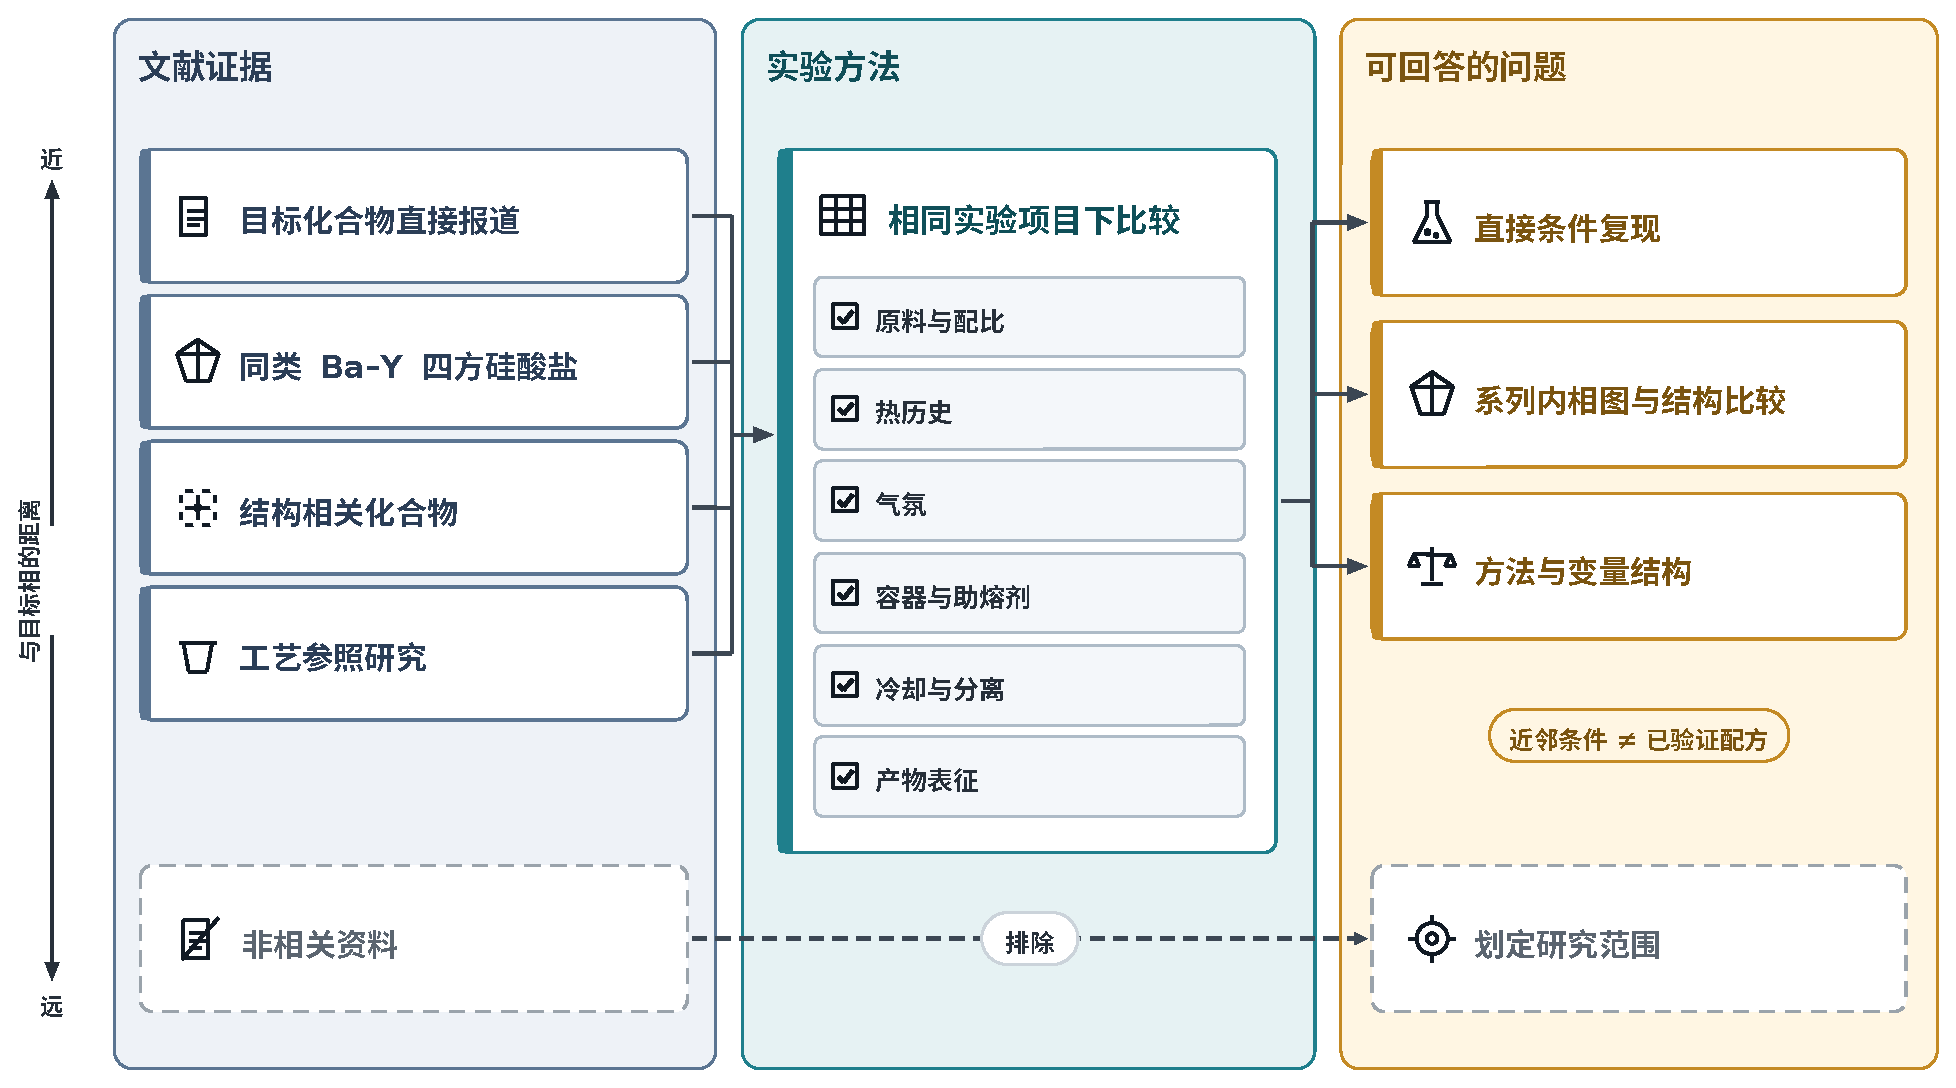
\includegraphics[width=\linewidth]{../figures/pdf/fig01_evidence_synthesis_map.pdf}
  \caption[不同文献对目标化合物合成研究的适用范围]{不同文献对目标化合物合成研究的适用范围。左侧依次列出目标化合物直接报道、同类Ba--Y四方硅酸盐、结构相关化合物、工艺参照研究和非相关资料；中间按相同实验项目整理原料、热史、气氛、容器、冷却和产物表征；右侧说明各类资料能够回答的问题。目标化合物直接报道目前只有一篇\cite{ababaikeri2024ba5y12zn}。相关体系的数值只用于说明实验变量和表征方法，不能直接作为目标相的已验证配方。}
  \label{fig:evidence-map}
\end{figure}

图~\ref{fig:evidence-map}表示文献对象、实验条件与可回答问题的对应关系。先确认文献实际研究的相，再在相同实验项目下比较原料、热史、气氛、容器和冷却条件。这样的整理有助于比较，但不消除化合物之间的结构差异。文献与目标相越远，可借鉴的内容越限于变量设置、实验设计和表征方法，具体温度、配比或助熔剂用量不能直接移用。

\subsection{结构相关性}

结构相关性至少要求有可追溯的晶体学证据，不能只看元素是否相同。Ba$M$SiO$_4$（$M=$Co、Zn、Mg）经单晶X射线和粉末中子衍射归入stuffed-tridymite衍生结构族\cite{liu1993structures}。该结果可比较Zn、Mg和Co四面体网络，但该族缺少Y且结构谱系不同，不能作为目标相的直接依据。BaZn$_2$Si$_2$O$_7$的低温和高温结构经中子与X射线衍射区分\cite{lin1999phase}；Ba$_2$ZnSi$_2$O$_7$的单斜结构由单晶精修确立\cite{kaiser2002crystal}；BaZnSi$_3$O$_8$的衍射结果展示了ZnO$_4$与SiO$_4$的连接网络\cite{zou2021crystal}。这些研究有助于确定待比较的结构参数，但不能回答目标相应在何种条件下复现。

Ba--Si--O体系中四配位Si网络的复杂性和热响应可作外围结构参照\cite{gorelova2016thermal}。Y$_2$Si$_2$O$_7$多型及其热膨胀资料表明，同一组成可能对应不同结构；跨年代比较必须核对结构模型和观察温度\cite{dolan2008structures,becerro2004revision}。这些结果可用于提出结构表征问题，但不提供目标相的稳定区间。

综上，同类Ba--Y研究可检验组成和相区，结构相关研究可比较位点和表征方法，工艺参照研究可完善实验设计。具体合成条件只能在原始研究对象和实验范围内解释，不能因化合物“相似”而直接外推。

\subsection{不适用资料的边界}

仅含Ba和Si并不足以构成结构相关性。Benitoite型BaSi$_4$O$_9$的结构精修\cite{finger1995refinement}、高压BaSi$_4$O$_9$的三方结构\cite{hazen1999crystal}、tribarium silicate的精修\cite{tillmanns1978refinement}以及高温Ba$_2$[Si$_4$O$_{10}$]的结构记录\cite{katscher1973the}，都显示Ba--Si--O网络可能具有不同结构，但缺少目标相所需的Y/Zn位点对应。高压Ba硅酸盐出现9R/6H钙钛矿型结构的记录进一步表明，压力路径可能通向另一类网络，也不能反推常压目标路线\cite{yusa2007rhombohedral}。

同样，功能语境相近也不能替代结构证据。Ce$^{3+}$掺杂Ba$_5$Si$_8$O$_{21}$的光学研究没有提供Y/Zn目标身份\cite{zhong2020combining}；非中心对称LiBa$_2$GaSi$_2$O$_8$与目标相共享光学语境，却不具备相同组成或结构谱系\cite{gu2025liba2gasi2o8}。Stuffed-silica的经典概念和零热膨胀材料的理论—实验综述可以帮助统一术语、理解热机械行为，但不能支持目标相的配方判断\cite{buerger1954the,erlebach2020thermomechanical}。

因此，非相关资料只用于划定研究范围，不进入目标相的合成条件比较。即使把相关资料列在同一张表中，表格也只表示实验项目可比较，不表示不同化合物具有相同结构或成相条件。
